\documentclass[a4paper,12pt]{article}

\renewcommand\thesection{\arabic{section}.}

\usepackage{tocloft}
\cftsetindents{section}{0em}{2em}
\cftsetindents{subsection}{0em}{2em}
\renewcommand\cfttoctitlefont{\hfill\Large\bfseries}
\renewcommand\cftaftertoctitle{\hfill\mbox{}}
\setcounter{tocdepth}{2}

\usepackage{listings}
\usepackage{xcolor}

\usepackage{fullpage}

\usepackage{float}

\usepackage{amsfonts}

\usepackage{titlesec}
\titlelabel{\thetitle.\quad}

\usepackage{sectsty}
\sectionfont{\fontsize{14}{15}\selectfont}

% to remove numbering in section, but not in subsections
\renewcommand{\thesection}{}
\renewcommand{\thesubsection}{\arabic{section}.\arabic{subsection}}
\makeatletter
\def\@seccntformat#1{\csname #1ignore\expandafter\endcsname\csname the#1\endcsname\quad}
\let\sectionignore\@gobbletwo
\let\latex@numberline\numberline
\def\numberline#1{\if\relax#1\relax\else\latex@numberline{#1}\fi}
\makeatother

\setcounter{tocdepth}{4}
\setcounter{secnumdepth}{4}

\usepackage{graphicx}
\usepackage{wrapfig}
\usepackage[left=1.75cm,right=1.75cm,top=2cm,bottom=1cm,includefoot,headsep=0.1in]{geometry}

\usepackage{fancyhdr}
\pagestyle{fancy}
\fancyhf{}
\cfoot{\thepage}

\usepackage{booktabs}
\usepackage{tabularx}

\usepackage[hidelinks]{hyperref}
\renewcommand{\refname}{\large CHAPTER 6: REFERENCES}
\usepackage[nottoc,numbib]{tocbibind}

%\usepackage{array}
%\newcolumntype{P}[1]{>{\centering\arraybackslash}p{#1}}

\lstset { %
	% basicstyle=\ttfamily,
  	% columns=fullflexible,
  	% frame=single,
  	breaklines=true,
  	postbreak=\mbox{\textcolor{red}{$\hookrightarrow$}\space},
    language=python,
    backgroundcolor=\color{black!5}, % set backgroundcolor
    basicstyle=\large,% basic font setting
}

\newcommand*{\plogo}{\fbox{$\mathcal{PL}$}} % Generic publisher logo

%----------------------------------------------------------------------------------------
%	TITLE PAGE
%----------------------------------------------------------------------------------------

\newcommand*{\titleGM}{\begingroup % Create the command for including the title page in the document
\hbox{ % Horizontal box
\hspace*{0.15\textwidth} % Whitespace to the left of the title page
\rule{1pt}{\textheight} % Vertical line
\rule{1pt}{\textheight}
\hspace*{0.03\textwidth} % Whitespace between the vertical line and title page text
\parbox[b]{0.75\textwidth}{ % Paragraph box which restricts text to less than the width of the page

{\noindent\Huge\bfseries Project Report}\\[2\baselineskip] % Title
{\large \textit{-supervised by:}\\\\\Large \textsc Dr. Ratan K. Ghosh\\\\Dr. Subhajit Sidhanta}\\[4\baselineskip] % Tagline or further description

{\large \textit{-submitted by:}\\\\\Large \textsc{Rohit Das \large{(11910230), and}}} % Author name
{\\\\\Large \textsc{Shoumik Ghosal \large{(11910300)}}} % Author name
\vspace{15em} % Whitespace between the title block and the publisher
\begin{figure}[H]
\hspace*{100pt}

\includegraphics[width=10em,height=\textheight,keepaspectratio]{./img/iitbhilai.png}
\end{figure}

\vspace{2em}
{\noindent \textbf {\Large{Indian Institute of Technology, Bhilai\\\\CS525\\\\}March \hspace{5pt}2020}}\\[\baselineskip] % Publisher and logo
}}
\endgroup}

\begin{document}
\thispagestyle{empty}
\titleGM % This command includes the title page

\large \tableofcontents

\clearpage
\section*{\large Declaration}
\label{sec:declaration}
\addcontentsline{toc}{section}{\nameref{sec:declaration}}

{\Large We declare that this written submission represents our ideas in our own words and where others' ideas or words have been included, we have adequately cited and referenced the original sources. We also declare that we have adhered to all principles of academic honesty and integrity and have not misrepresented or fabricated or falsified any idea/data/fact/source our submission. We understand that any violation of the above will be cause for disciplinary action by the Institute and can also evoke penal action from the sources which have thus not been properly cited or from whom proper permission has not been taken when needed.}

\vspace{7.5em}

\hspace{4em} \textsc{Rohit Das \hspace{10em} Shoumik Ghoshal}

\hspace{4em} \textsc{(11910230) \hspace{11.5em} (11910300)}

\clearpage
\section*{\large ABSTRACT}
\label{sec:abstract}
\addcontentsline{toc}{section}{\nameref{sec:abstract}}

{\large P2P file sharing is the process of sharing digital content like electronic books, multimedia (music, movies, video clips) through a direct connection between two peers or nodes over the P2P network. This is done with the help of a P2P client software which allows a computer to get connected to a P2P network. The peer which hosts the file is called a seed and the one which downloads it is called a leech. With the introduction of the BitTorrent\cite{bittorrent} protocol, files can be easily shared between peers via seeders, without overloading a single file server. DHT, or distributed hash tables, are a unique way of keeping track of file-owners, or their neighbours. Kademlia\cite{kademlia} is a routing algorithm which optimizes this search for the nearest neighbour using DHTs.

Here we present a peer-to-peer file-sharing system using DHTs instead of trackers,i.e. servers where information of nodes, seeders, etc. are stored. Kademlia is used to optimize the search in DHTs for nodes having the full or partial file(s), and efficiently get the IP and Port of such nodes.}

\clearpage
\section{\large CHAPTER 1: INTRODUCTION}

\subsection{P2P File-Sharing:}

\subsubsection{What is P2P File-Sharing?}
Peer-to-peer\cite{p2p} file sharing is the distribution and sharing of digital media using peer-to-peer (P2P) networking technology. P2P file sharing allows users to access media files such as books, music, movies, and games using a P2P software program that searches for other connected computers on a P2P network to locate the desired content.

A peer-to-peer network allows computer hardware and software to communicate without the need for a server. Unlike client-server architecture, there is no central server for processing requests in a P2P architecture. The peers directly interact with one another without the requirement of a central server.

Now, when one peer makes a request, it is possible that multiple peers have the copy of that requested object. Now the problem is how to get the IP addresses of all those peers. This is decided by the underlying architecture supported by the P2P systems. By means of one of these methods, the client peer can get to know about all the peers which have the requested object/file and the file transfer takes place directly between these two peers.

\subsubsection{Types of P2P Architecture:}

There are roughly three such architectures:
\begin{itemize}
\itemsep0em

\item Centralized Directory

\item Query Flooding

\item Exploiting Heterogeneity

\end{itemize}

\paragraph{Centralized Directory:}

\begin{wrapfigure}{R}{0.5\textwidth}
\centering
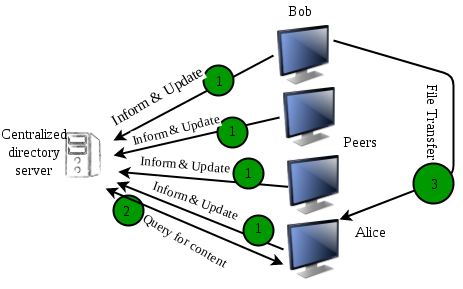
\includegraphics[width=0.45\textwidth]{./img/p2p-1.png}
\caption{\label{fig:p2p-1} Centralized Directory}
\end{wrapfigure}

It maintains a huge central server to provide directory service. All the peers inform this central server of their IP address and the files they are making available for sharing. The server queries the peers at regular intervals to make sure if the peers are still connected or not. This server maintains a huge database regarding which file is present at which IP addresses.

Now whenever a requesting peer comes in, it sends its query to the server. Since the server has all the information of its peers, so it returns the IP addresses of all the peers having the requested file to the peer. Now the file transfer takes place between these two peers.

\paragraph{Query Flooding:}

\begin{wrapfigure}{L}{0.45\textwidth}
\centering
\includegraphics[width=0.42\textwidth]{./img/p2p-2.png}
\caption{\label{fig:p2p-2}Query Flooding}
\end{wrapfigure}

Unlike the centralized approach, this method makes use of distributed systems. In this, the peers are supposed to be connected into an overlay network. It means if a connection/path exists from one peer to other, it is a part of this overlay network. In this overlay network, peers are called as nodes and the connection between peers is called an edge between the nodes, thus resulting in a graph-like structure.

Now when one peer requests for some file, this request is sent to all its neighboring nodes i.e. to all nodes which are connected to this node. If those nodes don’t have the required file, they pass on the query to their neighbors and so on. This is called as query flooding. When the peer with requested file is found (referred to as query hit), the query flooding stops and it sends back the file name and file size to the client, thus following the reverse path. If there are multiple query hits, the client selects from one of these peers.

\paragraph{Exploiting Heterogeneity:}

\begin{wrapfigure}{R}{0.45\textwidth}
\centering
\includegraphics[width=0.4\textwidth]{./img/p2p-3.png}
\caption{\label{fig:p2p-3} Supernodes}
\end{wrapfigure}

This P2P architecture makes use of both the above discussed systems. It resembles a distributed system like Gnutella because there is no central server for query processing. But it does not treat all its peers equally. The peers with higher bandwidth and network connectivity are at a higher priority, called as group leaders/super nodes. The rest of the peers are assigned to these super nodes. These super nodes are interconnected and the peers under these super nodes inform their respective leaders about their connectivity, IP address and the files available for sharing.

This structure can process the queries in two ways. The first one is that the super nodes could contact other super nodes and merge their databases with its own database. Thus, this super node now has information of a large number of peers. Another approach is that when a query comes in, it is forwarded to the neighboring super nodes until a match is found. Thus query flooding exists but with limited scope as each super node has many child peers. Hence, such a system exploits the heterogeneity of the peers by designating some of them as group leaders/super nodes and others as their child peers.


\subsection{Distributed Hash Tables (DHTs):}

A distributed hash table (DHT) is a distributed system that provides a lookup service similar to a hash table: $\langle$key, value$\rangle$ pairs are stored in a DHT, and any participating node can efficiently retrieve the value associated with a given key. Nodes can be added/removed with minimum work around re-distributing keys. Keys are unique identifiers which map to particular values, which in turn can be anything from addresses, to documents, to arbitrary data. Responsibility for maintaining the mapping from keys to values is distributed among the nodes, in such a way that a change in the set of participants causes a minimal amount of disruption. This allows a DHT to scale to extremely large numbers of nodes and to handle continual node arrivals, departures, and failures.

DHTs characteristically emphasize the following properties:
\begin{itemize}
\itemsep0em

\item Autonomy and decentralization: the nodes collectively form the system without any central coordination.

\item Fault tolerance: the system should be reliable (in some sense) even with nodes continuously joining, leaving, and failing.

\item Scalability: the system should function efficiently even with thousands or millions of nodes.

\end{itemize}

\begin{wrapfigure}{L}{0.6\textwidth}
\centering
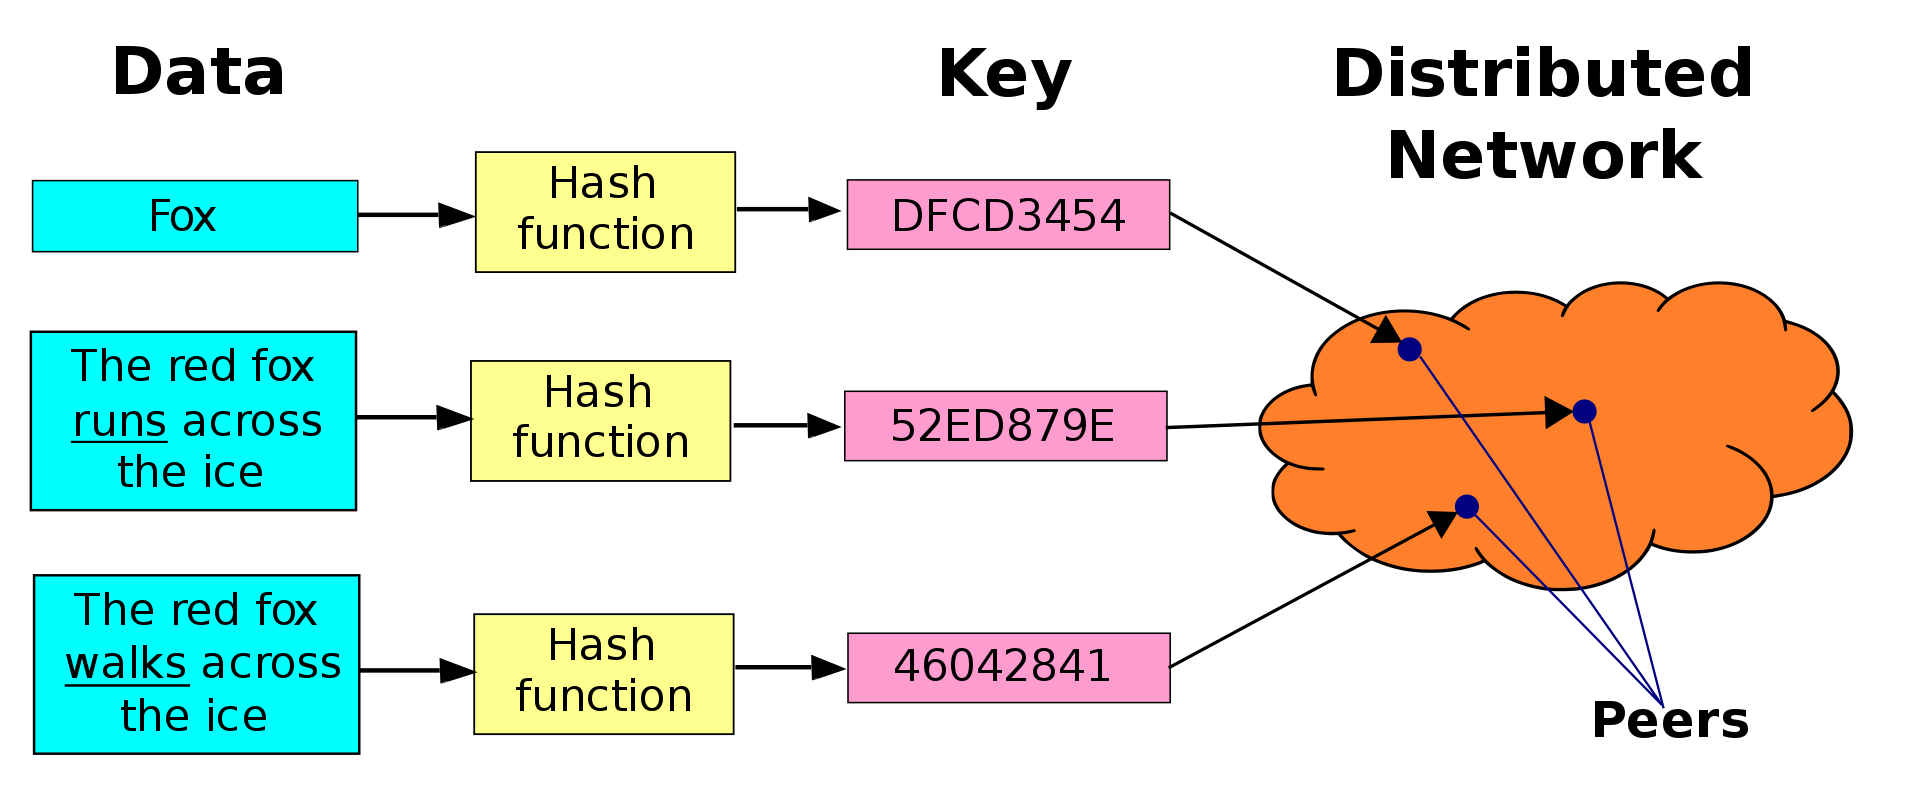
\includegraphics[width=0.55\textwidth]{./img/dht.png}
\caption{\label{fig:dht}Distributed Hash Tables}
\end{wrapfigure}

Any one node needs to coordinate with only a few other nodes in the system -- most commonly, $O(log n)$ of the $n$ participants -- so that only a limited amount of work needs to be done for each change in membership.

Some DHT designs seek to be secure against malicious participants and to allow participants to remain anonymous, though this is less common than in many other peer-to-peer (especially file sharing) systems.

Finally, DHTs must deal with more traditional distributed systems issues such as load balancing, data integrity, and performance (in particular, ensuring that operations such as routing and data storage or retrieval complete quickly).

\clearpage
\section{\large CHAPTER 2: LITERATURE SURVEY}

\subsection{BitTorrent Protocol:}

BitTorrent is a protocol for distributing files. It identifies content by URL and is designed to integrate seamlessly with the web. Its advantage over plain HTTP is that when multiple downloads of the same file happen concurrently, the downloaders upload to each other, making it possible for the file source to support very large numbers of downloaders with only a modest increase in its load. A BitTorrent file distribution consists of the following entites:

\begin{itemize}
\itemsep0em

\item An ordinary web server

\item A static `metainfo' server

\item A BitTorrent tracker

\item An `original' downloader

\item The end user downloaders

\end{itemize}

\subsubsection{Bencoding:}

Bencoding is the encoding used to store metadata in a .torrent file. Strings are length-prefixed base ten followed by a colon and the string. For example \texttt{4:spam} corresponds to `spam'. Integers are represented by an 'i' followed by the number in base 10 followed by an 'e'. For example \texttt{i3e} corresponds to 3 and \texttt{i-3e} corresponds to -3. Integers have no size limitation. \texttt{i-0e} is invalid. All encodings with a leading zero, such as \texttt{i03e}, are invalid, other than \texttt{i0e}, which of course corresponds to 0. 

Lists are encoded as an 'l' followed by their elements (also bencoded) followed by an 'e'. For example \texttt{l4:spam4:eggse} corresponds to ['spam', 'eggs']. Dictionaries are encoded as a 'd' followed by a list of alternating keys and their corresponding values followed by an 'e'. For example, \texttt{d3:cow3:moo4:spam4:eggse} corresponds to \{'cow': 'moo', 'spam': 'eggs'\} and \texttt{d4:spaml1:a1:bee} corresponds to \{'spam': ['a', 'b']\}. Keys must be strings and appear in sorted order (sorted as raw strings, not alphanumerics).

\subsubsection{Peer Protocol:}

BitTorrent's peer protocol operates over TCP or uTP. Peer connections are symmetrical. Messages sent in both directions look the same, and data can flow in either direction. The peer protocol refers to pieces of the file by index as described in the metainfo file, starting at zero. When a peer finishes downloading a piece and checks that the hash matches, it announces that it has that piece to all of its peers. Connections contain two bits of state on either end: choked or not, and interested or not. Choking is a notification that no data will be sent until unchoking happens.

Data transfer takes place whenever one side is interested and the other side is not choking. Interest state must be kept up to date at all times - whenever a downloader doesn't have something they currently would ask a peer for in unchoked, they must express lack of interest, despite being choked. This makes it possible for downloaders to know which peers will start downloading immediately if unchoked. Connections start out choked and not interested. When data is being transferred, downloaders should keep several piece requests queued up at once in order to get good TCP performance. 

On the other side, requests which can't be written out to the TCP buffer are immediately queued up in memory rather than kept in an application-level network buffer, so they can all be thrown out when a choke happens. The peer wire protocol consists of a handshake followed by a never-ending stream of length-prefixed messages. The handshake starts with character ninteen (decimal) followed by the string 'BitTorrent protocol'. The leading character is a length prefix, put there in the hope that other new protocols may do the same and thus be trivially distinguishable from each other. All later integers sent in the protocol are encoded as four bytes big-endian. 

After the fixed headers come eight reserved bytes, which are all zero in all current implementations. If you wish to extend the protocol using these bytes, please coordinate with Bram Cohen to make sure all extensions are done compatibly. Next comes the 20 byte sha1 hash of the bencoded form of the info value from the metainfo file. (This is the same value which is announced as info{\_}hash to the tracker, only here it's raw instead of quoted here). If both sides don't send the same value, they sever the connection. After the download hash comes the 20-byte peer id which is reported in tracker requests and contained in peer lists in tracker responses. If the receiving side's peer id doesn't match the one the initiating side expects, it severs the connection.


\subsection{Kademlia and the XOR Metric:}

Kademlia minimizes the number of configuration messages nodes must send to learn about each other. It uses parallel, asynchronous queries to avoid timeout delays from failed nodes. While Kademlia takes the basic approach of many DHTs, like opaque, 160-bit keys, $\langle$key,value$\rangle$ pairs being stored in nodes with IDs ``close'' to the key, many of its benefits result from its use of a novel XOR metric for distance between points in the key space.

\subsubsection{System Description:}

\begin{figure}[H]
\centering
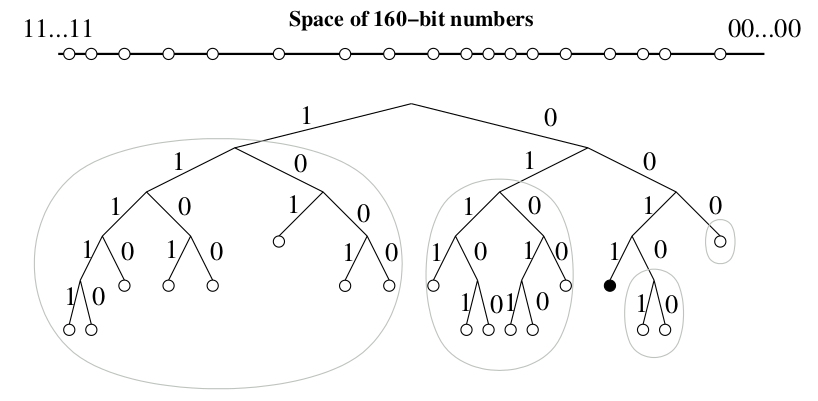
\includegraphics[width=0.75\textwidth]{./img/kadem-1.png}
\caption{\label{fig:kadem-1} Kademlia binary tree. The black dot shows the location of node 0011.... in the tree.}
\end{figure}

Kademlia effectively treats its nodes as leaves in a binary tree, with each node's position determined by the shortest unique prefix of its ID. For any given node, the binary tree is divided into a series of successively lower subtrees that don't contain the node. The highest subtree consists of the half of the binary tree not containing the node. The next subtree consists of the half of the remaining subtree not containing the node and so forth.

\subsubsection{XOR Metric:}

\begin{figure}[H]
\centering
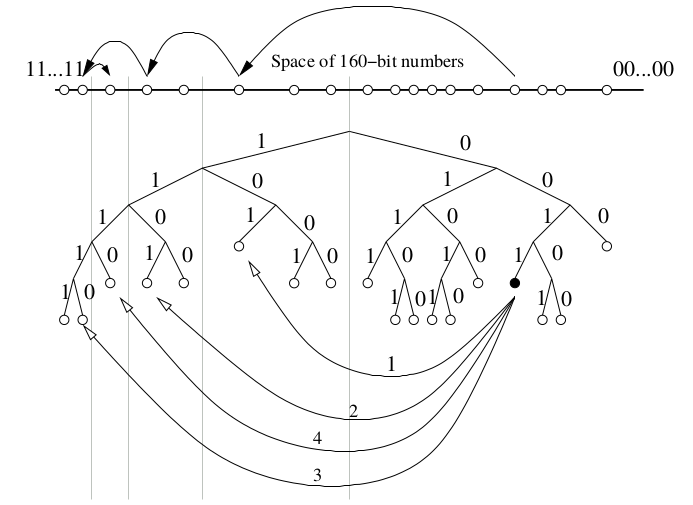
\includegraphics[width=0.75\textwidth]{./img/kadem-2.png}
\caption{\label{fig:kadem-2} Locating a node $1110$ by its ID.}
\end{figure}

Every message a node transmits includes its node ID, permitting the recipient to record the sender's existence if necessary. Kademlia relies on a notion of distance between two identifiers. Given two identifiers, $x$ and $y$, Kademlia defines the distance between them as ther bitwise exclusive or (XOR) interpreted as an integer, $d(x,y)$ = $x \oplus y$.

XOR captures the notion of distance implicit in the binary-tree-based sketch of the system. In a fully-populated binary tree of 160 bit IDs, the magnitude of the distance between two IDs is the height of the smallest subtree containing them both. When a tree is not fully populated, the closest leaf to an ID $x$ is the leaf whose ID shares the longest common prefix of $x$. If there are empty branches in the tree, there might be more than one leaf with the longest common prefix. In that case, the closest leaf to $x$ will be the closest leaf to ID $x$ produced by flipping the bits in $x$ corresponding to the empty branches of the tree.

\clearpage
\section{\large CHAPTER 3: METHODS DEVELOPED}

Here we have presented our implementation of parsing the .torrent file, and piece and block management while fetching and merging bytes of file downloaded. We also check the integrity of the pieces downloaded, block by block. We fixed the block size at $2^{14}$. All implementations have been done in python3.

\subsection{Bencode parsing:}
File: bencoding.py
\lstinputlisting[showstringspaces=false]{/home/mouri/MTech/CS525/Project/bit-torrent-dht/bencoding.py}

\subsection{Blocks and Pieces Management:}
File: blocks.py
\lstinputlisting[showstringspaces=false]{/home/mouri/MTech/CS525/Project/bit-torrent-dht/blocks.py}
\vspace{2em}
File: pieces.py
\lstinputlisting[showstringspaces=false]{/home/mouri/MTech/CS525/Project/bit-torrent-dht/pieces.py}
\vspace{2em}
File: piece{\_}mgr.py
\lstinputlisting[showstringspaces=false]{/home/mouri/MTech/CS525/Project/bit-torrent-dht/piece_mgr.py}

\clearpage
\section{\large CHAPTER 4: RESULTS AND CONCLUSIONS}

Pending further implementation and metric monitoring.

\clearpage
\section{\large CHAPTER 5: FUTURE SCOPE}

We are yet to implement message passing to indicate choked/unchoked, interested/not interested, and mainly, the DHT.

\clearpage
\bibliographystyle{unsrt}
\bibliography{References}

\end{document}